\documentclass[a4paper,11pt]{article}
\usepackage[spanish]{babel}
\usepackage[utf8]{inputenc}

% Configuración páginas
\usepackage{vmargin}							% Márgenes

\usepackage{sectsty}							% Fuente de los títulos
\allsectionsfont{\normalfont \Large \scshape}

\usepackage{graphicx}							% Imágenes
\graphicspath{{images/}}

\usepackage{tabularx}							% Otras tablas
\usepackage{listliketab}						% Tratar indentacion distas como tablas

\usepackage{mathtools}							% Matematicas
\newcommand\numberthis{							% numeración en align*
	\addtocounter{equation}{1}\tag{\theequation}
}

% Configuración del título
\newcommand{\horrule}[1]{\rule{\linewidth}{#1}} 	% Horizontal rule

\title{
	\vspace{-25pt}
	\normalfont \Large \textsc{
		Modelos de Investigación Operativa,
        Ingeniería Informática\\
        Universidad de Valladolid
	}\\[10pt]
	\horrule{1pt}\\[10pt]
	\huge \textbf{
		Práctica 15
	}\\
	\horrule{1pt}
}
\author{
	\normalfont \Large Daniel González Alonso
}
\date{
	\normalfont \large \today
}

%%%%%%%%%%%%%%%%%%%%%%%%%%%%%%%%%%%%%%%%%%%%%%%%%%
\begin{document}
\maketitle

%%%% RESUMEN %%%%
\begin{abstract}
	En este documento se describen los problemas y los resultados obtenidos de la práctica 15 del tema 6 de la asignatura Modelos de Investigación Operativa de Ingeniería Informática, Universidad de Valladolid.
\end{abstract}

%%%% DESARROLLO %%%%
\section{Introducción}
Esta práctica trata de problemas de Rutas de Vehículos Capacitado (CVRP, \textit{Capacited Vehicle Routing Problem}). Los problemas CVRP tratan determinar las rutas que una flota de vehículos ha de seguir con el fin de cubrir la demanda de todos sus clientes.\\

Los problemas CVRP constan de un grafo ${G=(V,A)}$, donde ${V}$ son los vértices del grafo y ${A}$ los arcos entre éstos, con un coste ${c_{i,j}}$ asociado a cada arco. El primer vértice del grafo es el depósito de partida de la flota de vehículos, mientras que los ${2 \ldots n}$ vértices restantes son los clientes a abastecer. Cada vértice del grafo tiene asociado una demanda ${d_{i} \geq 0}$, en el caso del depósito esta demanda es siempre ${d_{1}=0}$. Por otro lado, se supone que nuestra flota de vehículos es homogénea, es decir todos los vehículos tienen la misma capacidad, con un total de ${K}$ vehículos. También se supone que todos los punto de demanda pueden ser satisfechos y que la matriz de costes satisface la desigualdad triangular:

\begin{align*}\numberthis
	\label{desigualdad_triangular}
	c_{i,k} + c_{k,j} \geq c_{i,j}	&& \forall i,j,k \in V \\
\end{align*}

Para poder resolver este problema en la presente práctica, se han empleado dos modelos distintos:

\begin{enumerate}
\item \textbf{Modelo de dos índices}:
\begin{align*}\numberthis
   	&\textrm{Minimizar }	&& \sum_{i=1}^{n}{ \sum_{j=1}^{n}{c_{i,j} \cdot x_{i,j}} }	&& \\
   	&\textrm{Sujeto a }		&& \sum_{i=1}^{n}{x_{i,j}} = 1	&& j=2 \ldots n	\\
    &						&& \sum_{j=1}^{n}{x_{i,j}} = 1	&& i=2 \ldots n	\\
	&						&& \sum_{i=1}^{n}{x_{i,1}} = K	&& \\
    &						&& \sum_{i=j}^{n}{x_{1,j}} = K	&& \\
    &						&& \sum_{i \notin S}\sum_{j \in S}{x_{i,1}} \geq r(S)		&& \forall S \subseteq V-\{1\}, \ S \neq \emptyset \\
	&						&& x_{i,j} \in \{0,1\}			&& i=1 \ldots n, \ j = 1 \ldots n	\\
\end{align*}

En este problema primero hay que destacar la variable de decisión ${x_{i,j}}$ que nos indica si en la solución final se encuentra el arco ${(i,j)}$. En cuanto a las restricciones, la primera restricción y la segunda imponen respectivamente que de cada vértice cliente entre y salga solo un arco. La tercera y cuarta restricción imponen respectivamente que del vértice del depósito entren y salgan exactamente ${K}$ arcos. Por último la quinta restricción garantiza que se cumplan las restricciones de capacidad y la conectividad de la solución.

\item \textbf{Modelo de flujo de redes}: Este modelo a diferencia del anterior, no necesita conocer inicialmente el número de vehículos a utilizar. El modelo es el siguiente:

\begin{align*}\numberthis
   	&\textrm{Minimizar }	&& \sum_{i=1}^{n}{ \sum_{j=1}^{n}{c_{i,j} \cdot x_{i,j}} }	&& \\
   	&\textrm{Sujeto a }		&& \sum_{i=1}^{n}{x_{i,j}} = 1	&& j=2 \ldots n	\\
    &						&& \sum_{j=1}^{n}{x_{i,j}} = 1	&& i=2 \ldots n	\\
    &						&& \sum_{j=1}^{n}{y_{i,h}} - \sum_{j=1}^{n}{y_{j,i}} = b_{i}	&& i=1 \ldots n \\
    &						&& y_{i,j} \leq C \cdot x_{i,j}	&& i=1 \ldots n, \ j = 1 \ldots n	\\
    &						&& y_{i,j} \geq 0				&& i=1 \ldots n, \ j = 1 \ldots n	\\
	&						&& x_{i,j} \in \{0,1\}			&& i=1 \ldots n, \ j = 1 \ldots n	\\
\end{align*}

En este problema, además de las variables binarias de la solución ${x_{i,j}}$ tenemos las variables de flujo ${y_{i,j}}$. Inicialmente los valores de las variables ${b_{i}}$ es de ${-d_{i}, i=2 \ldots n}$ y para el vértice del depósito ${d_{1} = \sum_{j=2}^{n}{d_{j}}}$. Así mediante la tercera restricción aseguramos que no haya \textit{subtours} que no salgan del depósito. Por otro lado mediante la cuarta restricción impedimos que se supere la capacidad de los vehículos.
\end{enumerate}

\newpage
%%%%%%%%%%%%%%%%%%%%%%%%%%%%%%%%%%%%%%%%%%%%%%%%%%%%%%
\section{Desarrollo}
Para esta práctica se nos pide resolver los siguientes problemas:

\begin{enumerate}
\item Resolver un problema de distribución de gaseóleos mediante el modelo de dos índices y el de tres índices (ambos con número prefijado de vehículos), o el de dos índices y el de flujo en redes (ambos sin prefijar el número de vehículos).\\

En mi caso resolví este problema mediante el modelo de dos índices y el de flujo de redes sin fijar el número de vehículos. Los datos empleado para este problema se encuentran en el fichero \texttt{data/oil-delivery.dat}. El problema se resolvió mediante \textit{Xpress Mosel} en los ficheros \texttt{cvrp\_2\_indices\_oil\_delivery.mos} en el caso del modelo de dos índices, y en \texttt{cvrp\_redes\_oil\_delivery.mos} para el modelo de flujo de redes. En ambos casos se siguieron los esquemas expuestos en el apartado anterior, aunque cabe destacar que para el modelo de flujo de redes, para implementar la quinta restricción, ésta se sustituyó por una serie de restricciones de eliminación de \textit{subtours} de Miller:

\begin{align*}\numberthis
    &						&& u_{i} - u_{j} + C \cdot x_{i,j} \leq C - d_{j}	&& i,j=2 \ldots n \mid i \neq j,  \ d_{i} + d_{j} \leq C 	\\
	&						&& d_{i} \leq u_{i} \leq C		&& i=2 \ldots n	\\
\end{align*}

Siendo ${u_{i}}$ una variable continua que indica la cantidad de carga disponible en un vehículo después de visitar el vértice ${i}$.

\item Resolver un problema de recogida de residuos. Los datos de este problema se encuentran en el fichero \texttt{data/datos\_residuos.dat}.\\

Al igual que en el caso anterior se resolvió empleando el modelo de 2 índices (con las restricciones de Miller) y el modelos de flujo de redes en los ficheros \texttt{cvrp\_2\_indices\_ \ residuos.mos} y  \texttt{cvrp\_redes\_residuos.mos} respectivamente.

\item Resolver una serie de problemas con distancias Euclídeas mediante algún modelo exacto y resolverlo con Xpress, o con NEOS Server, con un tiempo límite de 100 segundos.\\

Los problemas en cuestión se encuentran en los ficheros \texttt{data/E021-04m.dat}, \texttt{data/ \ E026-08m.dat}, \texttt{data/E051-05e.dat} y \texttt{data/E076-10e.dat}. Todos estos problemas se resolvieron mediante \textit{Xpress Mosel} usando el modelo de flujo de redes en los ficheros \texttt{cvrp\_redes\_e021.mos}, \texttt{cvrp\_redes\_e026.mos}, \texttt{cvrp\_redes\_e051.mos} y \texttt{cvrp\_ \ redes\_e076.mos} (el nombre indica el fichero de datos empleado). Estos problemas se resolvieron de forma idéntica a los problemas implementados mediante los modelos de flujo de redes de los ejercicios anteriores, con la única diferencia de que en los ficheros de datos en vez de venir una matriz de costes o de distancias venían las coordenadas de cada vértice del grafo. Debido a esta diferencia, antes de aplicar el modelo se tuvo que calcular la matriz de costes a partir de las coordenadas empleando la distancia Euclídea redondeada al entero más cercano.
\end{enumerate}

%%%%%%%%%%%%%%%%%%%%%%%%%%%%%%%%%%%%%%%%%%%%%%%%%%%%%%
\section{Resultados}
Los resultados obtenidos a los problemas anteriores fueron los siguientes:

\begin{table}[!htbp]
\label{results_oil_delivery}
\centering
\begin{tabularx}{\textwidth}{|X|X|X|}
\hline
Modelo empleado	& Modelo de 2 índices	& Modelo de flujo de redes	\\ \hline
Solución	& 497	& 379	\\ \hline
Número de vehículos	& 2	& 4	\\ \hline
Valores de x (arcos)	& (1,3) (1,5) (2,7) (3,6) (4,1) (5,4) (6,2) (7,1)	& (1,1) (1,3) (1,4) (2,6) (3,2) (4,1) (5,1) (6,5) (7,7) \\ \hline
\end{tabularx}
\caption{Comparación de resultados para el fichero \texttt{oil-delivery.dat}}
\end{table}

\begin{table}[!htbp]
\label{results_residuos}
\centering
\begin{tabularx}{\textwidth}{|X|X|X|}
\hline
Modelo empleado	& Modelo de 2 índices	& Modelo de flujo de redes	\\ \hline
Solución	& 290	& 290	\\ \hline
Número de vehículos	& 4	& 4	\\ \hline
Valores de x (arcos)	& (1,2) (1,6) (1,8) (1,9) (2,3) (3,4) (4,5) (5,1) (6,1) (7,1) (8,13) (9,10) (10,7) (11,1) (12,11) (13,12)	& (1,5) (1,6) (1,7) (1,8) (2,1) (3,2) (4,3) (5,4) (6,1) (7,9) (8,11) (9,10) (10,1) (11,12) (12,13) (13,1)	\\ \hline
\end{tabularx}
\caption{Comparación de resultados para el fichero \texttt{ejemplo\_residuos.dat}}
\end{table}

\begin{table}[!htbp]
\label{results_e0}
\centering
\begin{tabularx}{\textwidth}{|X|X|X|X|X|}
\hline
Fichero de datos	& \texttt{E021-04m.dat}	& \texttt{E026-08m.dat}	& \texttt{E051-05e.dat}	& \texttt{E076-10e.dat}	\\ \hline
Nº de vértices	& 21	& 26	& 51	& 76	\\ \hline
Solución	& 358	& 606	& 584	& 918	\\ \hline
Nº de vehículos	& 5	& 9	& 7	& 12	\\ \hline
Valores de x (arcos)	& (1,1) (1,2) (1,8) (1,15) (1,18) (2,7) (3,1) (4,16) (5,1) (6,1) (7,20) (8,10) (9,3) (10,4) (11,13) (12,21) (13,1) (14,17) (15,14) (16,5) (17,19) (18,9) (19,11) (20,12) (21,6)	& (1,1) (1,3) (1,4) (1,13) (1,17) (1,18) (1,20) (1,24) (1,25) (2,7) (3,5) (4,1) (5,26) (6,8) (7,15) (8,1) (9,10) (10,1) (11,1) (12,9) (13,12) (14,22) (15,1) (16,1) (17,14) (18,6) (19,23) (20,16) (21,1) (22,21) (23,1) (24,2) (25,19) (26,11)	& (1,1) (1,12) (1,20) (1,32) (1,33) (1,38) (1,50) (2,28) (3,30) (4,29) (5,48) (6,1) (7,1) (8,44) (9,49) (10,39) (11,40) (12,17) (13,47) (14,26) (15,7) (16,45) (17,51) (18,13) (19,1) (20,41) (21,36) (22,35) (23,2) (24,8) (25,15) (26,19) (27,9) (28,1) (29,23) (30,21) (31,10) (32,27) (33,3) (34,46) (35,31) (36,37) (37,4) (38,18) (39,6) (40,34) (41,42) (42,14) (43,5) (44,25) (45,43) (46,16) (47,1) (48,1) (49,24) (50,11) (51,22)	& (1,1) (1,5) (1,13) (1,27) (1,34) (1,39) (1,46) (1,47) (1,49) (1,52) (1,59) (1,69) (2,44) (3,63) (4,45) (5,75) (6,16) (7,1) (8,54) (9,20) (10,1) (11,40) (12,1) (13,73) (14,53) (15,36) (16,58) (17,18) (18,4) (19,25) (20,55) (21,38) (22,31) (23,65) (24,64) (25,50) (26,51) (27,68) (28,76) (29,62) (30,6) (31,1) (32,56) (33,41) (34,74) (35,1) (36,1) (37,70) (38,1) (39,66) (40,10) (41,1) (42,57) (43,7) (44,42) (45,33) (46,30) (47,9) (48,37) (49,48) (50,1) (51,19) (52,17) (53,35) (54,12) (55,14) (56,26) (57,24) (58,28) (59,11) (60,15) (61,71) (62,22) (63,23) (64,1) (65,43) (66,67) (67,60) (68,8) (69,3) (70,72) (71,21) (72,61) (73,32) (74,2) (75,29) (76,1)	\\ \hline
\end{tabularx}
\caption{Resultados obtenidos para los ficheros \textit{e0}}
\end{table}

\newpage
Para el tercer problema además de los resultados se obtuvieron los gráficos IVE que representan los caminos de la solución a partir de las coordenadas dadas en los ficheros de datos:

\begin{figure}[!htbp]
	\centering
	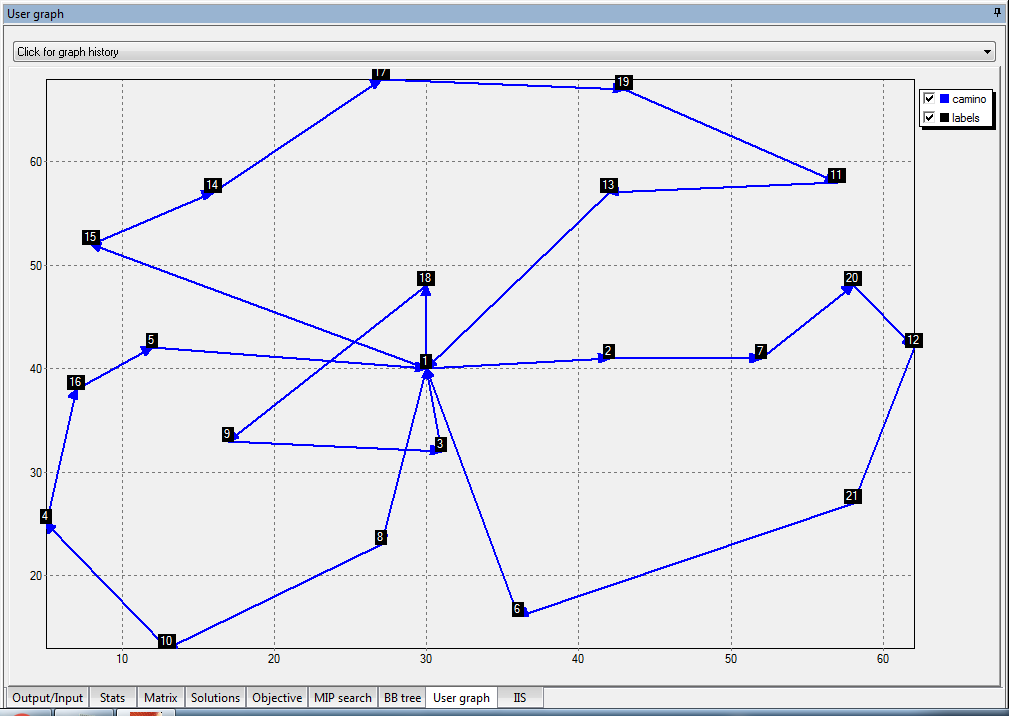
\includegraphics[width=1.0\textwidth, height=0.4\textheight]{e021_redes.png}
    \caption{Solución del problema \texttt{E021-04m.dat}}
\end{figure}

\begin{figure}[!htbp]
	\centering
	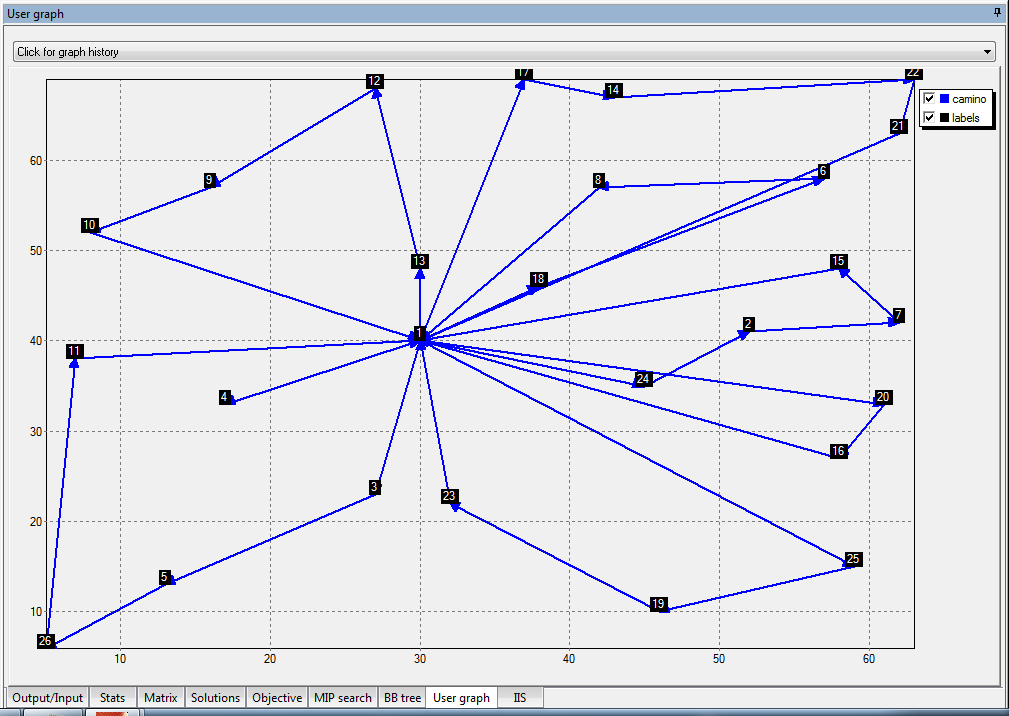
\includegraphics[width=1.0\textwidth, height=0.4\textheight]{e026_redes.png}
    \caption{Solución del problema \texttt{E026-08m.dat}}
\end{figure}

\begin{figure}[!htbp]
	\centering
	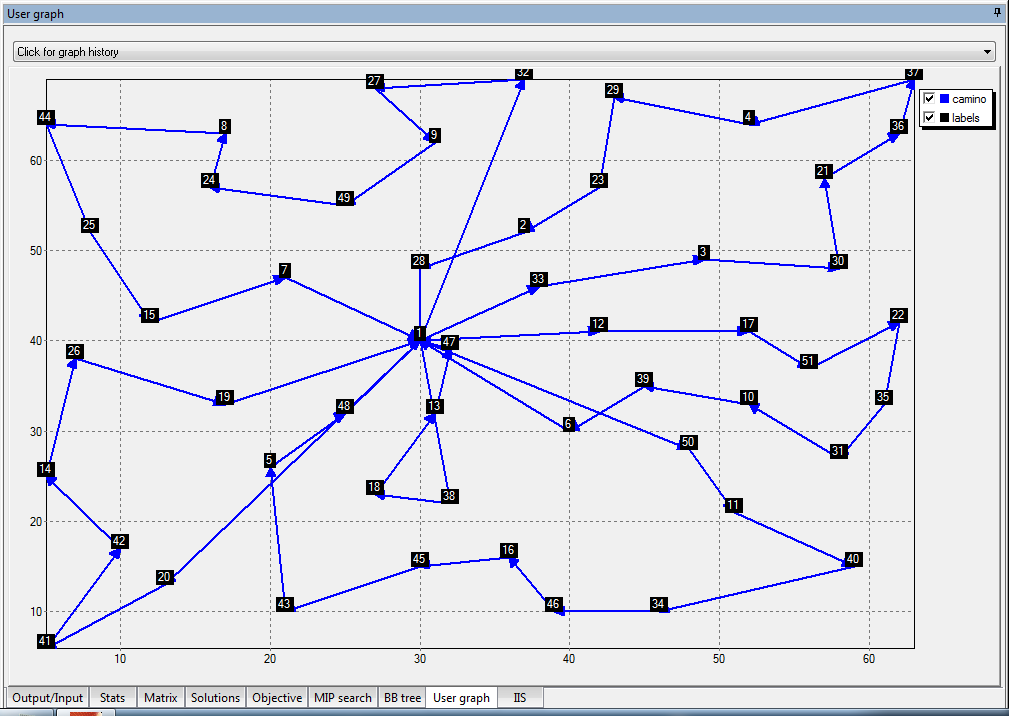
\includegraphics[width=1.0\textwidth, height=0.4\textheight]{e051_redes.png}
    \caption{Solución del problema \texttt{E051-05e.dat}}
\end{figure}

\begin{figure}[!htbp]
	\centering
	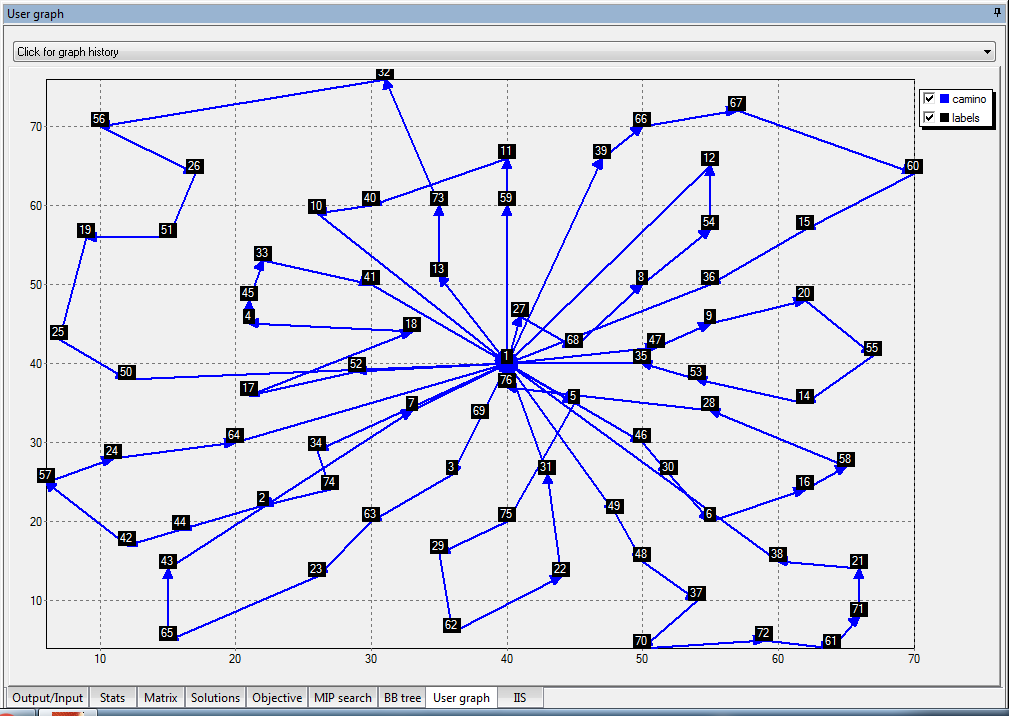
\includegraphics[width=1.0\textwidth, height=0.4\textheight]{e076_redes.png}
    \caption{Solución del problema \texttt{E076-10e.dat}}
\end{figure}

\end{document}
